\icode{E-MI-SI-L2-261111-002}
如图所示，两物块的质量分别为\(m_1\)和\(m_2\)。两轻质弹簧的劲度系数分别为\(k_1\)和\(k_2\)，上面木块压在上面的弹簧（但不栓接），整个系统处于平衡状态。现缓慢向上提上面的木块，直到它离开上面的弹簧。在这个过程中下面木块移动的距离为\paren[]

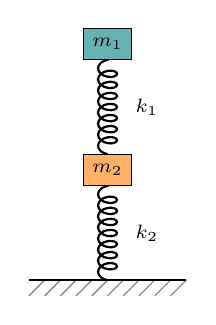
\begin{tikzpicture}[font=\scriptsize]
	\foreach \x in {-1,-.8,...,.8}
	\draw[gray] (\x,-.2)--++(.2,.2);
	\draw[thick] (-1,0)--(1,0);
	\draw[thick,decoration={aspect=.6,segment length=4,amplitude=1.2mm,coil},decorate] (0,0)--(0,1.2);
	\draw[fill=orange!60] (-.3,1.2) rectangle(.3,1.6)node[midway]{\(m_2\)};
    \draw[fill=teal!60] (-.3,2.8) rectangle(.3,3.2)node[midway]{\(m_1\)};
	\draw[thick,decoration={aspect=.6,segment length=4,amplitude=1.2mm,coil},decorate] (0,1.6)--(0,2.8);
	\node at(.5,.6){\(k_2\)};
	\node at(.5,2.2){\(k_1\)};
\end{tikzpicture}
\begin{choices}
	\item\(\frac{m_1g}{k_1}\)
	\item\(\frac{m_2g}{k_1}\)
	\item\(\frac{m_1g}{k_2}\)
	\item\(\frac{m_2g}{k_2}\)
\end{choices}
\begin{answer}
	C\qquad 提示：
\end{answer}